\documentclass{beamer}
%\documentclass[handout]{beamer}

\usetheme[language=english,framenumber,totalframenumber]{AlleghenyCollege}
\usepackage{tikz}
\usepackage{caption}

\title{Intelligent Monte-Carlo Tree Search for Perfect Information Games}
\author{Lucas Hawk}
\date{04/12/2017}

\begin{document}

\begin{frame}
  \titlepage
\end{frame}

%%%%%%%%%%%% Slide %%%%%%%%%%%%%%%%%%%%%%%%%%%%%%%%%%%%%%%%%%%%%%%%%%%

\begin{frame}
\frametitle{Presentation Overview}
\begin{enumerate}
\item Preliminaries
\item Implementation of Game-Playing Framework and Agents
\item Experimental Results
\begin{itemize}
\item Go Experiments
\item Hex Experiments (New!)
\end{itemize}
\item Future Work and Experimentation
\end{enumerate}
\end{frame}

%%%%%%%%%%%% Slide %%%%%%%%%%%%%%%%%%%%%%%%%%%%%%%%%%%%%%%%%%%%%%%%%%%
\begin{frame}
\frametitle{Motivation}
\onslide<1-> Perfect information games provide a very good environment for testing artificial intelligence.
\begin{itemize}
\onslide<2-> \item Extremely controllable
\onslide<2-> \item Clear goal for players
\onslide<2-> \item Simple programming, complex decision-making
\onslide<2-> \item Easy to benchmark agents both against each other and against humans
\end{itemize}
\end{frame}

%%%%%%%%%%%% Slide %%%%%%%%%%%%%%%%%%%%%%%%%%%%%%%%%%%%%%%%%%%%%%%%%%%
\begin{frame}
\frametitle{Monte-Carlo Tree Search (MCTS)}
MCTS is currently the “golden standard” for intelligent
game-playing agents
\begin{itemize}
\onslide<2-> \item ``Anytime algorithm"
\onslide<2-> \item Performance is game-independant --- MCTS does not use heuristics
\onslide<2-> \item Converges to optimal strategy
\end{itemize}
\end{frame}

%%%%%%%%%%%% Slide %%%%%%%%%%%%%%%%%%%%%%%%%%%%%%%%%%%%%%%%%%%%%%%%%%%
\begin{frame}
\frametitle{Monte-Carlo Tree Search (MCTS)}
\vspace{-0.75in}
\begin{center}
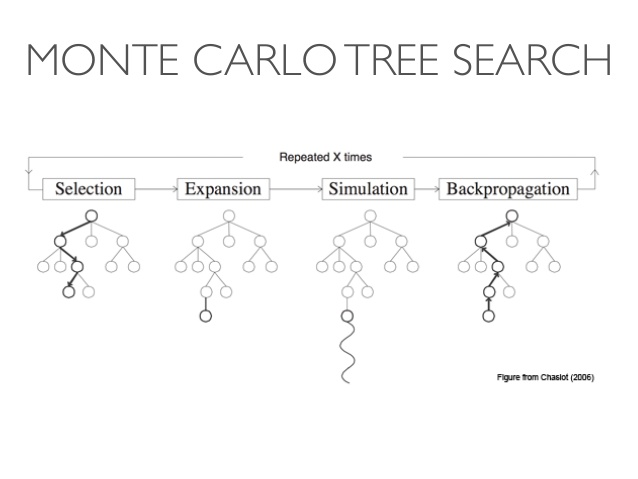
\includegraphics[clip, trim={0 4cm 0 5cm}, scale=.5]{images/mcts.jpg}
\end{center}
\end{frame}

%%%%%%%%%%%% Slide %%%%%%%%%%%%%%%%%%%%%%%%%%%%%%%%%%%%%%%%%%%%%%%%%%%
\begin{frame}
\frametitle{Why Go and Hex?}
Go and Hex are commonly used games in existing research
\begin{itemize}
\onslide<2-> \item Very small, simple ruleset
\onslide<2-> \item Very widely played
\onslide<2-> \item Massive branching factor
\begin{itemize}
\onslide<3-> \item 19x19 Go has $2 \times 10^{170}$ playouts, making it one of the most computationally complex board games ever created
\onslide<3-> \item Hex has a similar branching factor
\end{itemize}
\end{itemize}
\end{frame}

%%%%%%%%%%%% Slide %%%%%%%%%%%%%%%%%%%%%%%%%%%%%%%%%%%%%%%%%%%%%%%%%%%
\begin{frame}
\frametitle{Framework Implementation}
\vspace{-0.25in}
\begin{center}
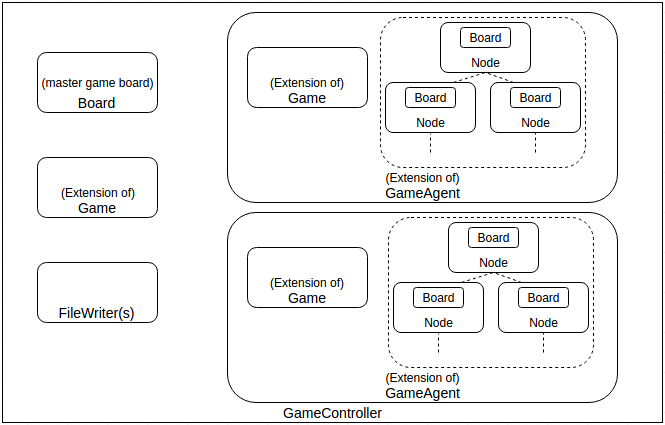
\includegraphics[scale=.35]{images/finalframework.png}
\end{center}
\end{frame}

%%%%%%%%%%%% Slide %%%%%%%%%%%%%%%%%%%%%%%%%%%%%%%%%%%%%%%%%%%%%%%%%%%
\begin{frame}
\frametitle{Agent Implementation}
\vspace{-0.25in}
\begin{figure}
\centering
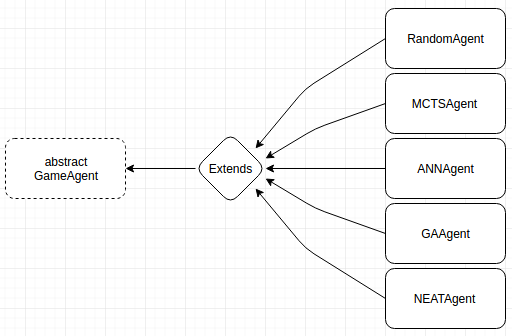
\includegraphics[scale=.35]{images/gameagent.png}
\caption*{Agent Inheritance Structure}
\end{figure}

\end{frame}

%%%%%%%%%%%% Slide %%%%%%%%%%%%%%%%%%%%%%%%%%%%%%%%%%%%%%%%%%%%%%%%%%%
\begin{frame}
\frametitle{Agent Implementation}
\vspace{-0.25in}
\begin{figure}
\centering
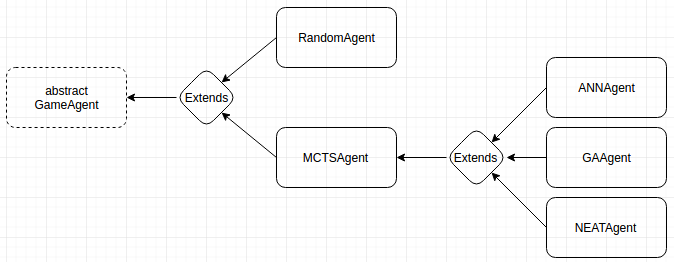
\includegraphics[scale=.35]{images/AgentShoulda.png}
\caption*{How it Should Have Worked}
\end{figure}

\end{frame}

%%%%%%%%%%%% Slide %%%%%%%%%%%%%%%%%%%%%%%%%%%%%%%%%%%%%%%%%%%%%%%%%%%
\begin{frame}
\frametitle{Intelligent Agents}
\begin{itemize}
\onslide<1-> \item ANNAgent
\onslide<2-> \item GAAgent
\onslide<3-> \item NEATAgent
\end{itemize}

\end{frame}

%%%%%%%%%%%% Slide %%%%%%%%%%%%%%%%%%%%%%%%%%%%%%%%%%%%%%%%%%%%%%%%%%%
\begin{frame}
\frametitle{Experiments}
\begin{itemize}
\onslide<1-> \item Compare performance of each agent when given a maximum time-allowed-per-move
\onslide<2-> \item Limiting time rather than MCTS iterations gives a more accurate indication of the tradeoff between complexity and performance
\end{itemize}
\end{frame}

%%%%%%%%%%%% Slide %%%%%%%%%%%%%%%%%%%%%%%%%%%%%%%%%%%%%%%%%%%%%%%%%%%
\begin{frame}
\frametitle{Experiments}
Experimental Setup
\begin{itemize}
\onslide<2-> \item Each pair of agents competed head-to-head in Hex and Go
\begin{itemize}
\onslide<3-> \item 9x9, 11x11, 14x14 Hex | 5x5, 7x7, 9x9, 11x11, 13x13 Go
\onslide<3-> \item Time-allowances of 500ms, 1000ms, 2000ms, 4000ms, 8000ms
\end{itemize}
\onslide<4-> \item 20 games of each combination of board size and time-allowance
\end{itemize}
\end{frame}

%%%%%%%%%%%% Slide %%%%%%%%%%%%%%%%%%%%%%%%%%%%%%%%%%%%%%%%%%%%%%%%%%%
\begin{frame}
\frametitle{Go Results vs RandomAgent}
\begin{center}
\begin{tabular}{|c|c|c|}
\hline
Agent (vs Random) & win rate & mean score (turn 250) \\ \hline \hline
MCTS & 98.8 & 33.1 \\ \hline
ANN & 98.4 & 32.5 \\ \hline
GA & 98.2 & 31.516 \\ \hline
\end{tabular}
\end{center}
\end{frame}

%%%%%%%%%%%% Slide %%%%%%%%%%%%%%%%%%%%%%%%%%%%%%%%%%%%%%%%%%%%%%%%%%%
\begin{frame}
\frametitle{Go Results vs RandomAgent}
\begin{figure}[h]
\centering
\begin{minipage}{.45\textwidth}
  \centering
  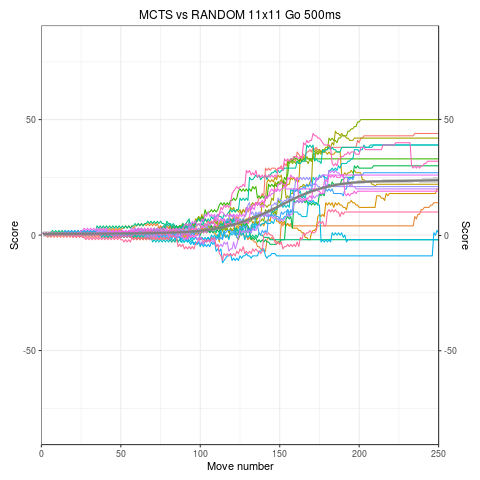
\includegraphics[scale=0.3]{images/mctsrand500go11.png}
\end{minipage}%
\begin{minipage}{.45\textwidth}
  \centering
  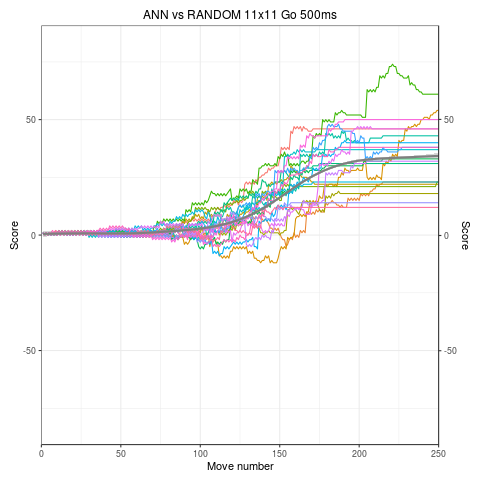
\includegraphics[scale=0.3]{images/annrand500go11.png}
\end{minipage}
\label{fig:rand}
\end{figure}
\end{frame}

%%%%%%%%%%%% Slide %%%%%%%%%%%%%%%%%%%%%%%%%%%%%%%%%%%%%%%%%%%%%%%%%%%
\begin{frame}
\frametitle{Go Results vs RandomAgent}
\centering
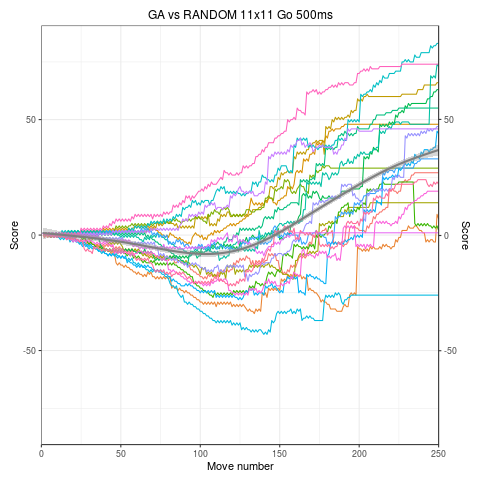
\includegraphics[scale=0.35]{images/garand500go11.png}
\end{frame}

%%%%%%%%%%%% Slide %%%%%%%%%%%%%%%%%%%%%%%%%%%%%%%%%%%%%%%%%%%%%%%%%%%
\begin{frame}
\frametitle{Go Results vs RandomAgent}
\begin{figure}[h]
\centering
\begin{minipage}{.45\textwidth}
  \centering
  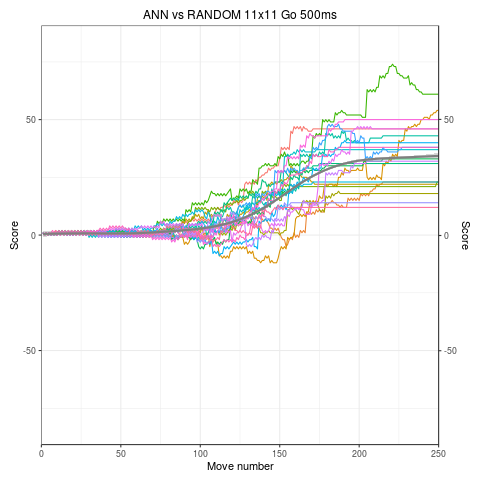
\includegraphics[scale=0.3]{images/annrand500go11.png}
\end{minipage}%
\begin{minipage}{.45\textwidth}
  \centering
  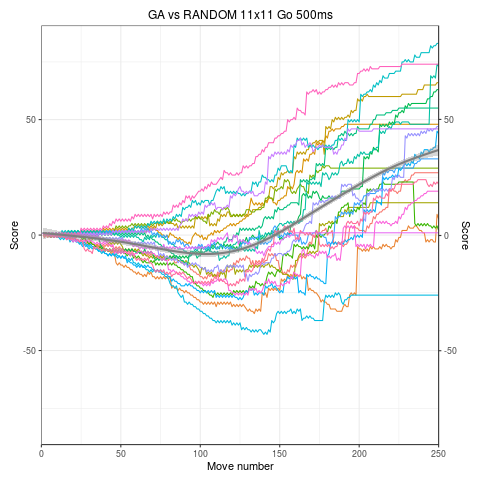
\includegraphics[scale=0.3]{images/garand500go11.png}
\end{minipage}
\label{fig:rand}
\end{figure}
\end{frame}

%%%%%%%%%%%% Slide %%%%%%%%%%%%%%%%%%%%%%%%%%%%%%%%%%%%%%%%%%%%%%%%%%%
\begin{frame}
\frametitle{Go Results vs MCTSAgent}
\begin{center}
\begin{tabular}{|c|c|c|}
\hline
Agent (vs MCTS) & win rate & mean score (turn 250) \\ \hline \hline
ANN & 61.4 & 4.31 \\ \hline
GA & 56.9 & 1.8 \\ \hline
\end{tabular}
\end{center}
\end{frame}

%%%%%%%%%%%% Slide %%%%%%%%%%%%%%%%%%%%%%%%%%%%%%%%%%%%%%%%%%%%%%%%%%%
\begin{frame}
\frametitle{Go Results vs MCTSAgent}
\begin{center}
Mean Score by time-allowance
\begin{tabular}{|c|c|c|}
\hline
time-allowance & GAAgent mean score & ANNAgent mean score \\ \hline \hline
1000 & -2.475 & 5.875 \\ \hline
2000 & -0.125 & 5.0 \\ \hline
4000 & 2.65 & 4.21 \\ \hline
8000 & 4.425 & 4.35 \\ \hline
\end{tabular}
\end{center}
\end{frame}

%%%%%%%%%%%% Slide %%%%%%%%%%%%%%%%%%%%%%%%%%%%%%%%%%%%%%%%%%%%%%%%%%%
\begin{frame}
\frametitle{Go Results vs MCTSAgent}
\begin{center}
Mean Score by board size
\begin{tabular}{|c|c|c|}
\hline
board size & GAAgent mean & ANNAgent mean \\ \hline \hline
5 & 2.86 & 1.41 \\ \hline
7 & 2.23 & 2.18 \\ \hline
9 & 1.81 & 4.39 \\ \hline
11 & -2.45 & 9.31 \\ \hline
\end{tabular}
\end{center}
\end{frame}

%%%%%%%%%%%% Slide %%%%%%%%%%%%%%%%%%%%%%%%%%%%%%%%%%%%%%%%%%%%%%%%%%%
\begin{frame}
\frametitle{Go Results Head2Head}
\begin{center}
GAAgent vs ANNAgent mean score by \\time-allowance and board size

\begin{tabular}{|c|c|||c|c|}
\hline
time-allowance & mean score & board size & mean score \\ \hline \hline
500 & -1.53 & 5 & 1.8\\ \hline
1000 & -1.7 & 7 & 2.47\\ \hline
2000 & -5.16 & 9 & -1.26\\ \hline
4000 & 1.41 & 11 & -5.8\\ \hline
8000 & 3.5 & --- & ---\\ \hline
\end{tabular}
\end{center}
\end{frame}

%%%%%%%%%%%% Slide %%%%%%%%%%%%%%%%%%%%%%%%%%%%%%%%%%%%%%%%%%%%%%%%%%%
\begin{frame}
\frametitle{Go Results Summary}
\begin{itemize}
\onslide<1-> \item GAAgent shows a positive correlation with time-allowance, and a negative correlation with board size
\onslide<2-> \item ANNAgent performance is more independant of time-allowance, board size than standard MCTSAgent
\onslide<3-> \item NEATAgent results still to come
\end{itemize}
\end{frame}

%%%%%%%%%%%% Slide %%%%%%%%%%%%%%%%%%%%%%%%%%%%%%%%%%%%%%%%%%%%%%%%%%%
\begin{frame}
\frametitle{Hex Results (new!)}
\begin{itemize}
\onslide<1-> \item Against the RandomAgent, both ANNAgent and MCTSAgent won $100\%$ of their games
\onslide<2-> \item GAAgent only won about $60\%$ of its games against RandomAgent
\end{itemize}
\end{frame}

%%%%%%%%%%%% Slide %%%%%%%%%%%%%%%%%%%%%%%%%%%%%%%%%%%%%%%%%%%%%%%%%%%
\begin{frame}
\frametitle{Hex Results vs MCTSAgent}
\begin{center}
\begin{tabular}{|c|c|}
\hline
Agent (vs MCTS) & win rate \\ \hline \hline
ANN & 66.6 \\ \hline
GA & 19.3 \\ \hline
\end{tabular}
\end{center}
\end{frame}

%%%%%%%%%%%% Slide %%%%%%%%%%%%%%%%%%%%%%%%%%%%%%%%%%%%%%%%%%%%%%%%%%%
\begin{frame}
\frametitle{Hex Results Head2Head}
\begin{itemize}
\onslide<1-> \item ANNAgent won $88\%$ of the 300 total games played
\onslide<2-> \item No trends regarding board size or time-allowance --- ANNAgent was simply dominant all around
\end{itemize}
\end{frame}

%%%%%%%%%%%% Slide %%%%%%%%%%%%%%%%%%%%%%%%%%%%%%%%%%%%%%%%%%%%%%%%%%%
\begin{frame}
\frametitle{Hex Results Summary}
\begin{itemize}
\onslide<1-> \item ANNAgent seems to perform similarly as in Go, providing a moderate performance boost with little correlation to board size or time-allowance
\onslide<2-> \item GAAgent \underline{SUCKS} (with the heuristic features we used)
\begin{itemize}
\onslide<3-> \item Highlights the agent's dependency on a valid, high-performance heuristic
\end{itemize}
\end{itemize}

\end{frame}

\begin{frame}
\frametitle{Results Summary}
\begin{itemize}
\item Even with a ``lightly trained" network, an agent using ANN pruning is able to outperform an agent using standard MCTS by $20$-$25\%$
\item ANN pruning performance seems to be independant of board size and time-allowance
\end{itemize}
\end{frame}

\begin{frame}
\frametitle{Results Summary}
\begin{itemize}
\onslide<1-> \item An agent utilizing a rapidly evolving GA is \textit{capable} of outperforming an agent using standard MCTS, or even the agent using ANN pruning
\onslide<2-> \item Agent's performance strongly correlates with both board size and time-allowance
\onslide<3-> \item Agent's performance is almost entirely dependant on a well-defined heuristic strategy of the game it is playing
\end{itemize}
\end{frame}

\begin{frame}
\frametitle{Future Work}
By the end of the semester
\begin{itemize}
\onslide<1-> \item NEATAgent evaluation
\onslide<2-> \item Analyze differences in computational complexity by looking at number of iterations per second each agent is able to complete
\end{itemize}

\onslide<3-> Beyond the end of the semester
\begin{itemize}
\onslide<3-> \item Go board resolution optimization
\onslide<3-> \item Effect of better-trained networks on ANNAgent performance
\end{itemize}
\end{frame}
\end{document}